\documentclass[12pt, a4paper]{scrartcl}


\usepackage{lmodern} 		% Diese beiden packages sorgen für echte 
\usepackage[T1]{fontenc}	% Umlaute.
\usepackage[utf8]{inputenc} 
\usepackage[ngerman]{babel}

\usepackage[pdfpagelabels,pdfstartview = FitH,bookmarksopen = true,bookmarksnumbered = true,linkcolor = black,plainpages = false,hypertexnames = false,citecolor = black, breaklinks]{hyperref}
\usepackage{url}
\usepackage{picins}


%Spezialpakete Zeichnen
\usepackage{tikz}
\usepackage{fp}
\usepackage{xcolor}
% TikZ-Bibliotheken
\usetikzlibrary{arrows}
\usetikzlibrary{shapes}
\usetikzlibrary{decorations.pathmorphing}
\usetikzlibrary{decorations.pathreplacing}
\usetikzlibrary{decorations.shapes}
\usetikzlibrary{decorations.text}


%%FIGUR
%\begin{figure}[htbp]
%\centering
%\includegraphics[width=15cm]{Bild1}%
%\caption{Experimental set-up}%
%\label{1}
%\end{figure}

%%BILD MIT PICINS NEBEN TEXT SETZEN
%\piccaption{Caption\label{label}} 
%\parpic[r]{\fbox{\includegraphics [width=5cm, keepaspectratio]{bild.png}}}
%


%% ZWEI BILDER NEBENEINANDER.
%% Schau, dass die minipages insgesamt nie mehr als 1.0\textwidth haben.
%% Um ein drittes oder viertes Bild einzufügen, ergänze einfach um weitere minipages.
% \begin{figure}[!htb]
% \centering
%   \minipage{0.3\textwidth}
%     \fbox{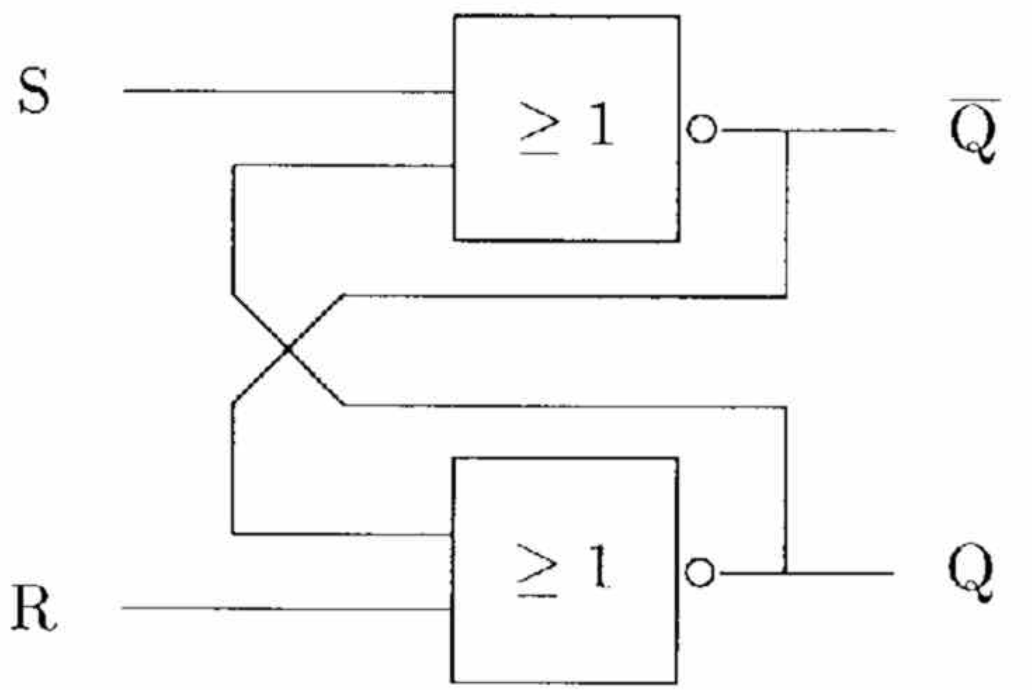
\includegraphics[height=2.5cm, keepaspectratio]{rsflipflop.png}}%
%     \caption{RS-Flipflop}%
%     \label{fig:rsflipflop}
%   \endminipage\hspace{1cm}   
% %
%   \minipage{0.4\textwidth}
%     \fbox{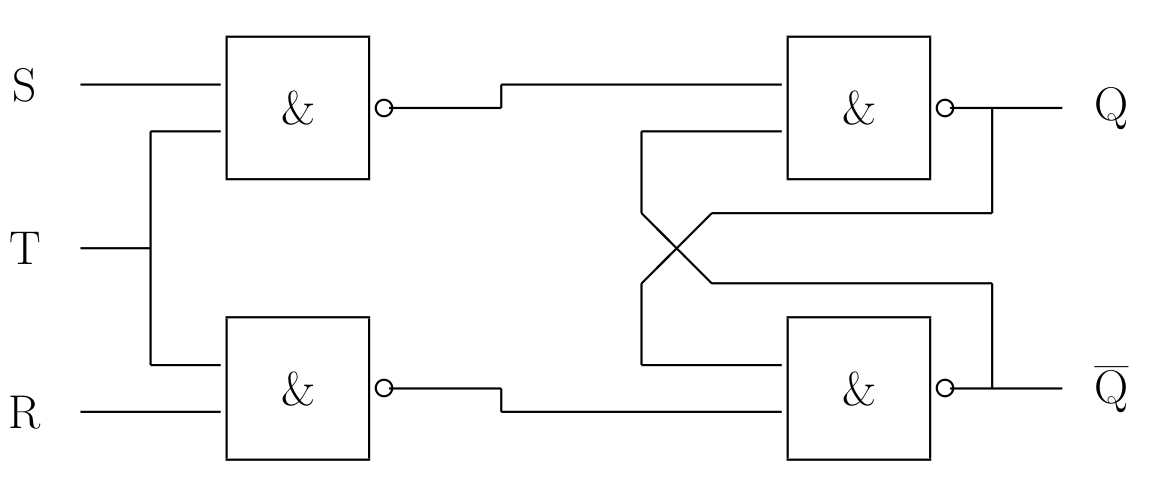
\includegraphics[height=2.5cm, keepaspectratio]{rsflipfloptakt.png}}%
%     \caption{getaktetes RS-Flipflop}%
%     \label{fig:rsflipfloptakt}
%   \endminipage
% \end{figure}




%------------------------------------------


\begin{document}

\section*{Drawing in \LaTeX}
\tableofcontents
\pagebreak

\subsection{Notizen}

\begin{verbatim}
% Spezialpakete
\usepackage{tikz}
\usepackage{fp}
\usepackage{tikz}
\usepackage{xcolor}
% TikZ-Bibliotheken
\usetikzlibrary{arrows}
\usetikzlibrary{shapes}
\usetikzlibrary{decorations.pathmorphing}
\usetikzlibrary{decorations.pathreplacing}
\usetikzlibrary{decorations.shapes}
\usetikzlibrary{decorations.text}

Command:
\tikz[options]{tikz commands}
\end{verbatim}

oder

\begin{verbatim}
   \begin{tikzpicture}
      blabla
   \end{tikzpicture}

\end{verbatim}


\begin{itemize}
   \item Innerhalb der tikzpicture-Umgebung keine leeren Zeilen!
   
   \item Wenn keine Grösse angegeben, werden die Werte in Klammern als $cm$ interpretiert.
   
   \item Das Koordinatensystem beginnt in der unteren linken Ecke der Arbeitsfläche.

   \item Benutze nicht Einheiten, sondern skaliere das Gesamtbild. Und falls nötig, zeige den Rechteck der Arbeitsfläche an.
   \begin{verbatim}
   \usetikzlibrary{backgrounds}
   \begin{tikzpicture}[scale=.8, show background rectangle]
   \end{verbatim}
      
   \item Falls Text in Nodes vorhanden ist: benutze 
   \begin{verbatim}
    \begin{tikzpicture}[scale=.9, transform shape]
    \end{verbatim} Transform shape: Damit Node-Text mitskaliert wird.

\end{itemize}

\subsection{Links}
\begin{itemize}
   \item \url{http://www.math.uni-leipzig.de/~hellmund/LaTeX/pgf-tut.pdf}
   \item \url{http://www.math.tugraz.at/~huss/new/teaching/computermathematik09/dateien/tikz_demonstration.pdf}
   \url{http://www.texample.net/tikz/}
   \item \url{https://www.sharelatex.com/blog/2013/08/27/tikz-series-pt1.html}
\end{itemize}




\pagebreak
\section{Basics}
\subsection{Gerade Linien zeichnen, relative Koordinaten}
\begin{tikzpicture}
\draw (0,0) -- (2, 2);
\end{tikzpicture}
%
\hspace{1cm}
%
\begin{tikzpicture}
   \draw (0,0) -- +(6.2, 0.7);
\end{tikzpicture}



\subsection{Pfeile}
\begin{tikzpicture}
\draw[->] (0,0) -- (2, 2);
% mit "+" werden relative Koordinaten angegeben
\draw[<->>, line width=3pt] (2,0) -- +(2, 2);
\draw[->, line width=2pt] (4,0) -- +(1, 1.5);
\draw[<-, red, dashed, line width = 2pt] (6,2) -- (8,0);
\draw[->, blue, dotted, line width = 2pt] (8,0) -- (10,3);
\end{tikzpicture}

{\renewcommand{\arraystretch}{2}%
\begin{tabular}{l l }
\begin{tikzpicture}
\draw[->] (0,0) -- (2,0);
\end{tikzpicture} & $\backslash draw[->]$ \\

\begin{tikzpicture}
\draw[dotted, >->>](0,0) -- (2,0);
\end{tikzpicture} & $\backslash draw[dotted, >->>]$\\

\begin{tikzpicture}
\draw[|<->|] (0,0) -- (2,0);
\end{tikzpicture} & $\backslash draw[|<->|]$\\

\begin{tikzpicture}
\draw[loosely dashed] (0,0) -- (2,0);
\end{tikzpicture} & $\backslash draw[loosely\ dashed]$\\

\begin{tikzpicture}
\draw[densely dotted] (0,0) -- (2,0);
\end{tikzpicture} & $\backslash draw[densely \ dotted]$ \\

\begin{tikzpicture}
\draw[->] (0,0) .. controls (.4,-.4) .. (2, 0);
\end{tikzpicture} & $\backslash draw[->] (0,0) .. controls (.4,-.4) .. (2, 0)$
\end{tabular}


\subsection{Polarkoordinaten; Geschlossene Figur}

\begin{verbatim}
   Polarkoordinaten: (winkel:radius). Winkel auch negativ möglich
   Zum Anfangspunkt verbinden: -- cycle;
\end{verbatim}
\begin{tikzpicture}
\draw (0:1cm) -- (72:1cm) -- (2*72:1cm) --
(3*72:1cm) -- (4*72:1cm) -- cycle;
\end{tikzpicture}
%
\hspace{2cm}
%
\begin{tikzpicture}
   \draw[blue, line width = 2pt] (0:1.5cm) -- (60:1.5cm) -- (2*60:1.5cm) -- (3*60:1.5cm) -- (4*60:1.5cm) --(-60:1.5cm) -- cycle;
\end{tikzpicture}
%
\hspace{2cm}
%
\begin{tikzpicture}
\draw[color=red] (0,0) -- (40:1);
\draw[color=blue] (0,0) -- (160:1);
\draw[thick] (0,0) -- (90:1);

\end{tikzpicture}


\subsection{Einfache Figuren}
\begin{tikzpicture}
   \draw (0, 0) rectangle (2, 1);
   \draw[color=red] (4, 0) circle (.5);
   \draw (6, 0) ellipse (.7 and 0.5);
\end{tikzpicture}






\section{Komplexeres}

\subsection{Fills}

\begin{tikzpicture}
\fill (0,0) circle (0.25);
\fill[red] (1,0) circle (0.25);
\fill[blue] (2,0) circle (0.25);
\shade[ball color=green] (3,0) circle (0.25);
\fill[orange] (4,0) circle (0.25);
\fill[green,opacity=0.5] (4.25,0) circle (0.25);
\end{tikzpicture}

\subsection{Clipping und Scope}
After a clip command, all subsequent drawings are clipped, only the parts inside the clipping region are drawn.

Use the scope environment to restrict the effect of clipping.

\begin{tikzpicture}
\draw (-2, 1.5) rectangle (2, -1.5);
\begin{scope}
\clip (-0.5, 0) circle (1); % Über clips wird eine abgeschlossene Fläche definiert. Sobald diese gemacht ist, wird nur noch das gezeichnet, was innerhalb dieser Fläche liegt, sonst nichts.
\clip ( 0.5, 0) circle (1);
\fill[color=gray!40] (-2,1.5)
rectangle (2,-1.5);
\end{scope} % Scope begrenzt die Wirkung des clippings. Alles ausserhalb von scope wird wieder gezeichnet.
\draw (-0.5, 0) circle (1);
\draw ( 0.5, 0) circle (1);
\end{tikzpicture}

\subsection{Kurvenlinien}
\begin{tikzpicture}
  \draw[line width = 2pt] (0,0) .. controls (2,1) and (4,-2) .. (8,0);
  \draw[dotted] (0,0)--(8,0);
\end{tikzpicture}

\begin{tikzpicture}
% Direkte eingabe der Kontrollpunkte:
\draw (0,0) .. controls (0,1) and (1,1) .. (2, 2);
% Die Line krümmt sich um 30 Grad nach Links:
\draw[bend left=30] (3,0) to (4, 2);
% aus- und eingehenden Winkel festlegen:
\draw (6,0)  to [out=90, in=-90] (7, 2) to [out = 20, in = -90] (10, 1);
\end{tikzpicture}

\subsection{Nodes}

\begin{verbatim}
\node[Options] (node name) at (x,y) {TeX content of node}
\end{verbatim}

\begin{tikzpicture}[scale=.9, transform shape] %Transform shape: Damit Nodes mitskaliert werden.
\tikzstyle{every node} = [circle, fill=gray!30]
\node (a) at (0, 0) {A};
\node (b) at +(0: 1.5) {B};
\node (c) at +(60: 1.5) {C};
\foreach \from/\to in {a/b, b/c, c/a}
\draw [->] (\from) -- (\to);
\end{tikzpicture}

\begin{tikzpicture}
\node (A) at (0,0) [circle,shade,draw] {$\sin(x)$};
\node (B) at (3,0) {$\cos(x)$};
\node (C) at (6,0) [fill=red!50] {$-\sin(x)$};
\draw[->, blue!50, very thick] (A) to[bend right=20]
node[above] {$\frac{\partial}{\partial x}$} (B);
\draw[->, blue!50, very thick] (B) to (C);
\draw[<->, thick] (A) to[out=45, in=135] (C);
\end{tikzpicture}



\section{Varia}
\subsection{grid}
\begin{tikzpicture}
\draw[step=1cm,gray,very thin] (-1,-1) grid (2,2);
\end{tikzpicture}
%
\begin{tikzpicture}
\draw[step=0.5cm,gray,very thin] (-1.5,-1.5) grid (1.5,1.5);
\end{tikzpicture}
%
\begin{tikzpicture}
\draw[step=1mm,gray,very thin] (-1.5,-1.5) grid (1.5,1.5);
\end{tikzpicture}

\subsection{Axes}
\begin{tikzpicture}
\draw[step=1cm,gray!20,very thin] (-1.9,-1.9) grid (5.9,5.9);
\draw[thick,->] (0,0) -- (4.5,0) node[anchor=north west] {x axis};
\draw[thick,->] (0,0) -- (0,4.5) node[anchor=south east] {y axis};
\foreach \x in {0,1,2,3,4}
\draw (\x cm,1pt) -- (\x cm,-1pt) node[anchor=north] {$\x$};
\foreach \y in {0,1,2,3,4}
\draw (1pt,\y cm) -- (-1pt,\y cm) node[anchor=east] {$\y$};
\end{tikzpicture}

%
\subsection{Color fillings}
\begin{tikzpicture}
\filldraw[fill=blue!40!white, draw=black] (0,0) rectangle (2,2);
\end{tikzpicture}
%
%
\begin{tikzpicture}
\shade[left color=blue,right color=red] (0,0) rectangle (2,2);
\end{tikzpicture}
%
\begin{tikzpicture}
\shade[top color=blue,bottom color=red] (0,0) rectangle (2,2);
\end{tikzpicture}
%
\begin{tikzpicture}
\shadedraw[inner color=blue,outer color=red, draw=black] (0,0) rectangle (2,2);
\end{tikzpicture}


\vfill
\newpage
\section{Meine Zeichnungen}
\subsection{Praktikumsbericht Kern- und Teilchenphysik: Positronenvernichtung}
\subsubsection{1}
\fbox{
	\begin{tikzpicture}[scale=0.6, every node/.style={scale=0.8}]
		%
		%22Na
		\draw[line width = 3pt] (0,10) -- node[above=1mm]{\Large{$^{22}$\textbf{Na}}} (4,10) node[right=1mm]{$\tau_{1/2} = 2.6$a};
		%
		%Ne angeregter Zustand
		\draw[line width = 3pt] (5,5) -- node[above]{$\tau_{1/2} = 3$ps} (9,5);
		%
		%Ne Grundzustand
		\draw[line width = 3pt] (5,0) -- node[below=1mm]{\Large{$^{22}$\textbf{Ne}}} (9,0);
		%
		%Photon
		\draw[line width = 1.5pt, decorate, decoration=snake] (7,4.9)-- node[right=1mm]{$E_\gamma = 1.275$ MeV} (7,0.2);
		\draw[->, line width = 1.5pt] (7,0.2)--(7,0.1);
		%
		%beta+ 90%
		\draw[->, line width = 1.5pt] (3,10) -- node[right=1mm]{$\beta^{+}$, 90$\%$} (4.9,5.1);
		%
		%beta+ 0.5%
		\draw[->, line width = 1.5pt, style = dashed] (3,10) -- node[left=1mm]{$\beta^{+}$, 0.05$\%$} (4.9,0.1);
	\end{tikzpicture}
}

\subsubsection{2}
	
\fbox{ % Second picture
	\begin{tikzpicture}[scale=0.5, every node/.style={scale=0.8}]
		%100MHz
		\draw[line width = 1.5pt] (0,11) -- +(0.5, 0)-- +(0.5, 0.5) -- + (1, 0.5) -- +(1, 0)--
		+(1.5, 0)-- +(1.5, 0.5) -- + (2, 0.5) -- +(2, 0)-- node[above=5mm]{100MHz}
		+(2.5, 0)-- +(2.5, 0.5) -- + (3, 0.5) -- +(3, 0)--
		+(3.5, 0)-- +(3.5, 0.5) -- + (4, 0.5) -- +(4, 0)--
		+(4.5, 0)-- +(4.5, 0.5) -- + (5, 0.5) -- +(5, 0)
		;
		%
		%1kHz
		\draw[line width = 1.5pt] (6.5,11) -- +(0.5, 0)-- +(0.5, 0.5) -- + (1, 0.5) -- +(1, 0)-- node[above=5mm]{1kHz}
		+(4.5, 0)-- +(4.5, 0.5) -- + (5, 0.5) -- +(5, 0)-- +(5.5,0);
		%
		%Pfeil 100MHz
		\draw[->, line width = 1.5pt] (2.5, 10.5) -- (2.5, 9.1);
		%
		%Pfeil 10kHz
		\draw[->, line width = 1.5pt] (9, 10.5) -- (9, 9.1);
		%
		%Prescaler
		\draw[] (1.1,8) rectangle +(2.8,1);
		\node[] at (2.5, 8.5) {Prescaler};
		%
		%Diskriminator
		\draw[] (6.9,8) rectangle +(4.2,1);
		\node[] at (9, 8.5) {Diskriminator};
		%
		%TAC
		\draw[] (4.825,4.5) rectangle +(1.8,1);
		\node[] at (5.75, 5) {TAC};
		%
		%ADC
		\draw[] (4.825,1.5) rectangle +(1.8,1);
		\node[] at (5.75, 2) {ADC};
		%
		%Rechner
		\draw[] (8.4,1.5) rectangle +(2.6,1);
		\node[] at (9.75, 2) {Rechner};
		%
		%Pfeil Diskriminator- TAC
		\draw[->, line width = 1.5pt] (9, 7.9) -- node[right=1mm]{Start} (6.6, 5.6);
		%
		%Pfeil Prescaler-TAC
		\draw[->, line width = 1.5pt] (2.5, 7.9) -- node[left=1mm]{Stopp} (4.8, 5.6);
		%
		%Pfeil TAC-ADC
		\draw[->, line width = 1.5pt] (5.75, 4.4) -- (5.75, 2.6);
		%
		%Pfeil ADC-Rechner
		\draw[->, line width = 1.5pt] (6.8, 2) -- (8.2, 2);
	\end{tikzpicture}
}


\subsubsection{3}

	
\begin{tikzpicture}
	 \node at (2,0) [draw,thick,minimum width=2cm,minimum height=1cm] {BaF$_2$-Detektor};
	 %
	 \node at (7.2,1.2) [draw,thick,minimum width=2cm,minimum height=1cm] {Verstärker};
	 %
	 \node at (7.2,-1.2) [draw,thick,minimum width=2.2cm,minimum height=1cm, text width = 2.2cm] {\small{Pulse Height Analyser}};
	 %
	 \node at (11,1.2) [draw,thick,minimum width=2cm,minimum height=1cm]{Delay};
	 %
	 \node at (11,-1.2) [draw,thick,minimum width=2cm,minimum height=1cm, text width = 2.4cm] {\small{Einkanal- diskriminator}};
	 %
	 \node at (14,0) [draw,thick,minimum width=2cm,minimum height=1cm] {ADC};
	 %
	 \node at (2,-2) [thick,minimum width=2cm,minimum height=1cm] {Hochspannung};
	 %
	 %Hochspannung
	 \draw[->, line width = 1.5pt, style=dashed] (2, -1.7) -- (2, -0.7);
	 %
	 %Detektor-Verstärker
	 \draw[->, line width = 1.5pt] (3.7,0) -- (4.5,0)--(4.5, 1.2)--(6, 1.2);
	 %
	 %Detektor-PHA
	 \draw[->, line width = 1.5pt] (4.5,0) -- (4.5, -1.2) -- (5.8, -1.2);
	 %
	 %Verstärker-Delay
	 \draw[->, line width = 1.5pt] (8.5, 1.2)--(9.8,1.2);
	 %
	 %PHA-EKDisrk
	 \draw[->, line width = 1.5pt] (8.6, -1.2)--(9.5,-1.2);
	 %
	 %Delay-ADC
	 \draw[->, line width = 1.5pt] (12.1, 1.2)--(14,1.2)--node[right=1mm]{Signal} (14, 0.6);
	 %
	 %EKDiskr - ADC
	 \draw[->, line width = 1.5pt] (12.4, -1.2)--(14,-1.2)--node[right=1mm]{Gate} (14, -0.6);
\end{tikzpicture}


\subsubsection{4}

\fbox{
   	\begin{tikzpicture}[scale=0.55, every node/.style={scale=0.55}]
	   	%QUELLE
	   	\draw[line width=1.5pt] (0, 0) circle (0.5) node [above = 4mm] {$^{22}Na$-Quelle};
	   	\fill[fill=gray]
	   	(0, 0) circle (0.3);
	   	%
	   	%Hintergrund RECHTS
	   	\fill[fill=blue!40] (1.5,0.5)--(4.5,-0.5)--(1.5,-0.5)--cycle;
	   	\fill[fill=green!40] (1.5,0.5)--(4.5,0.5)--(4.5,-0.5)--cycle;
	   	%
	   	%Hintergrung LINKS
	   	\fill[fill=blue!40] (-1.5,-0.5)--(-1.5,0.5)--(-4.5,-0.5)--cycle;
	   	\fill[fill=green!40] (-4.5,-0.5)--(-4.5,0.5)--(-1.5,0.5)--cycle;
	   	%
	   	%Hochspannugn
	   	\node at (0,2) [thick,minimum width=2cm,minimum height=1cm, ]{Hochspannung};
	   	%
	   	%Koinzidenzeinheit
	   	\node at (0,-6.6) [draw, thick,minimum width=3.5cm,minimum height=1cm, fill=blue!40]{Koinzidenzeinheit};
	   	%
	   	%ADC
	   	\node at (0,-8.9) [draw, thick,minimum width=3.5cm,minimum height=1cm]{ADC};
	   	%
	   	%Rechner
	   	\node at (5,-8.9) [draw, thick,minimum width=3cm,minimum height=1cm]{Rechner};
	   	%
	   	%Pfeil Koinzidenzeinheit - ADC
	   	\draw[->, line width=1.5pt] (0, -7.2) -- node[right = 1mm]{Gate}(0, -8.3);
	   	%
	   	%Pfeil ADC-Rechner
	   	\draw[->, line width=1.5pt] (1.8, -8.9) -- (3.4, -8.9);
	   	%
	   	%TAC
	   	\node at (-3.5,-11.2) [draw, thick,minimum width=3cm,minimum height=1cm, fill=green!40]{TAC};
	   	%
	   	%Pfeil TAC-ADC
	   	\draw[->, line width=1.5pt] (-3.5, -10.6) -- (-3.5, -8.9)-- node[above=1mm]{Signal} (-1.8, -8.9);
	   	
	   	%%%%%%%%%%%%%%%%%%%%%%%%%%%%%%%%%%%%%%
	   	%RECHTE SEITE
	   	%Detektor
	   	\node at (3,0) [draw,thick, text width = 2.7cm, minimum height=1cm,] {BaF$_2$-Detektor};
	   	\draw[fill=gray] (1.2, -0.35) rectangle (1.5, 0.35);
	   	%
	   	%Hochspannung Pfeil
	   	\draw[->, line width=1.5pt, style = dashed] (1.5,2) -- (3,2)-- (3, 0.6);
	   	%
	   	%Verstärker
	   	\node at (3, -2.4)  [draw,thick,minimum width=2.2cm,minimum height=1cm, text width = 2.7cm, align=center, fill=blue!40] {Verstärker, PHA};
	   	%
	   	%Pfeil Detektor-PHA
	   	\draw[->, line width=1.5pt] (3,-0.6) -- (3,-1.8);
	   	%
	   	%EKDiskr
	   	\node at (3, -4.8)  [draw,thick,minimum width=2.2cm,minimum height=1cm, text width = 2.7cm, align=center, fill=blue!40] {Einkanal-diskriminator};
	   	%
	   	%Pfeil PHA - EKDiskr
	   	\draw[->, line width=1.5pt] (3,-3) -- (3,-4.2);
	   	%
	   	%Pfeil EKDiskr-Koinzidenzeinheit
	   	\draw[->, line width=1.5pt] (3,-5.4) -- (3,-6.6) -- (1.8, -6.6);
	   	%
	   	% CDF
	   	\node at (7.5,0) [draw,thick, text width = 3cm, minimum height=1cm, fill=green!40, align=center] {Constant Fraction Diskriminator};
	   	%
	   	%Pfeil Detektor-CDF
	   	\draw[->, line width=1.5pt] (4.6,0) -- (5.8,0);
	   	%
	   	%Delay
	   	\node at (7.5, -2.4)  [draw,thick,minimum width=2.2cm,minimum height=1cm, text width = 2.7cm, align=center, fill=green!40] {Delay};
	   	%
	   	%Pfeil CDF-Delay
	   	\draw[->, line width=1.5pt] (7.5,-0.9) -- (7.5,-1.8);
	   	%
	   	%Pfeil Delay-TAC
	   	\draw[->, line width=1.5pt] (7.5,-3) -- (7.5,-11.2)-- node [above = 1mm]{Stopp} (-1.9, -11.2);
	   	%%%%%%%%%%%%%%%%%%%%%%%%%%%%%%%%%%%%%%
	   	%%%%%%%%%%%%%%%%%%%%%%%%%%%%%%%%%%%%%%
	   	%%%%%%%%%%%%%%%%%%%%%%%%%%%%%%%%%%%%%%
	   	%LINKE SEITE
	   	%Detektor
	   	\node at (-3,0) [draw,thick, text width = 2.7cm, minimum height=1cm,] {BaF$_2$-Detektor};
	   	\draw[fill=gray] (-1.2, -0.35) rectangle (-1.5, 0.35);
	   	%
	   	%Hochspannung Pfeil
	   	\draw[->, line width=1.5pt, style = dashed] (-1.5,2) -- (-3,2)-- (-3, 0.6);
	   	%
	   	%Verstärker
	   	\node at (-3, -2.4)  [draw,thick,minimum width=2.2cm,minimum height=1cm, text width = 2.7cm, align=center, fill=blue!40] {Verstärker, PHA};
	   	%
	   	%Pfeil Detektor-PHA
	   	\draw[->, line width=1.5pt] (-3,-0.6) -- (-3,-1.8);
	   	%
	   	%EKDiskr
	   	\node at (-3, -4.8)  [draw,thick,minimum width=2.2cm,minimum height=1cm, text width = 2.7cm, align=center, fill=blue!40] {Einkanal-diskriminator};
	   	%
	   	%Pfeil PHA - EKDiskr
	   	\draw[->, line width=1.5pt] (-3,-3) -- (-3,-4.2);
	   	%
	   	%Pfeil EKDiskr-Koinzidenzeinheit
	   	\draw[->, line width=1.5pt] (-3,-5.4) -- (-3,-6.6) -- (-1.8, -6.6);
	   	%
	   	% CDF
	   	\node at (-7.5,0) [draw,thick, text width = 3cm, minimum height=1cm, fill=green!40, align=center] {Constant Fraction Diskriminator};
	   	%
	   	%Pfeil Detektor-CDF
	   	\draw[->, line width=1.5pt] (-4.6,0) -- (-5.8,0);
	   	%
	   	%Pfeil CDF-TAC
	   	\draw[->, line width=1.5pt] (-7.5,-0.9) -- (-7.5,-11.2)-- node [above=1mm]{Start}(-5.1,-11.2);
   	\end{tikzpicture}
}


\subsection{Proseminar Theoretische Physik: The Theory of Stellar Evolution}

\subsubsection{1}
\fbox{
\begin{tikzpicture}[scale=1, transform shape]
	%draw radii
	\draw[color=darkgray!70, line width=1pt] (0:0) arc (70:110:10); %lower radius
	\draw[color=darkgray!70, line width=1pt] (90:3) arc (70:110:10); %upper radius
	
	%main body of cylinder
	\draw[fill=gray!10] (-4.9,0.5) rectangle (-1.9, 3.5);
	\draw[color=darkgray!80] (-4.9,0.5) rectangle (-1.9, 3.5);
	%
	%
	%draw ellipses (cylinder surface: dS)
	\fill[color=gray!30] (-3.4,0.5) ellipse (1.5 and .4); % lower ellipse x: -3.4; y: 0.6-ellipse_height/2 + minor uplifting
	\fill[color=gray!30] (-3.4,3.5) ellipse (1.5 and .4); % upper ellipse: lower ellipse + 3 for y
	\draw[color=darkgray!80] (-3.4,3.5) ellipse (1.5 and .4); % upper ellipse: lower ellipse + 3 for y
	%
	% LOWER ELLIPSE
	\begin{scope} % dashed half-ellipse
	\clip (-1.9, 0.9) rectangle (-4.9, 0.5);
	\draw[color=darkgray!80, dashed] (-3.4,0.5) ellipse (1.5 and .4); % lower ellipse x: -3.4; y: 0.6-ellipse_height/2 + minor uplifting	
	\end{scope}
	\begin{scope} % full half-ellipse
	\clip (-1.9, 0.1) rectangle (-4.9, 0.5);
	\draw[color=darkgray!80] (-3.4,0.5) ellipse (1.5 and .4); % lower ellipse x: -3.4; y: 0.6-ellipse_height/2 + minor uplifting	
	\end{scope}
	%
	% Text nodes
	\node[scale=1.3] (a) at (-3.4, 3.5) {$dS$};
	\node[scale=1.3] (b) at (-3.4, 0.5) {$dS$};
	\node[scale=1.3] (c) at (-6.6, 0.4) {$r$};
	\node[scale=1.3] (d) at (-6.3, 3.6) {$r+dr$};
	\node[scale=1.3] (e) at (-3.4, 2) {$\Delta m$};
	\node[blue!60, scale=1.3] (f) at (-5.2, 2) {$P$};
	\node[blue!60, scale=1.3] (g) at (-1.6, 2) {$P$};
	\node[anchor=west, color=blue!60, scale=1.3] (h) at (-3.4, 4.5) {$P(r+dr)$};
	\node[anchor=west, color=blue!60, scale=1.3] (i) at (-3.4, -0.5) {$P(r)$};
	\node[anchor=west, red!60, scale=1.6] (j) at (-6.1, -0.7) {$\frac{G m \Delta m}{r^2}$};
	%
	% Arrows
	\draw [->, line width = 1 pt, >=stealth, color=blue!60] (-3.4, -1) -- +(0,1); % P(r)
	\draw [->, line width = 1 pt, >=stealth, color=blue!60] (-3.4, 5) -- +(0,-1); % P(r+dr)
	\draw [->, line width = 1 pt, >=stealth, color=blue!60] (-6, 2.5) -- +(1,0); % P left upper
	\draw [->, line width = 1 pt, >=stealth, color=blue!60] (-6, 1.5) -- +(1,0); % P left lower
	\draw [->, line width = 1 pt, >=stealth, color=blue!60] (-0.8, 2.5) -- +(-1,0); % P right upper
	\draw [->, line width = 1 pt, >=stealth, color=blue!60] (-0.8, 1.5) -- +(-1,0); % P right lower
	\draw [->, line width = 1 pt, >=stealth, red!60] (-4,2) -- +(0,-3); % Grav
\end{tikzpicture}
}


\subsubsection{2}

\begin{tikzpicture}[scale=0.5]
	\draw[fill=red!30, color=red!30] (0,0) rectangle (2,10); %slab
	%
	% radiation arrows
	\draw[line width = 1pt, decorate, decoration=snake, color=blue!40] (-2.5,8.5)--  (-0.4, 8.5);
	\draw[line width = 1pt, ->, >=stealth, color=blue!40] (-0.4,8.5)--(-0.1,8.5);
	%
	\draw[line width = 1pt, decorate, decoration=snake, color=blue!40] (-2.5,6.5)--  (-0.4, 6.5);
	\draw[line width = 1pt, ->, >=stealth, color=blue!40] (-0.4,6.5)--(-0.1,6.5);
	%
	\draw[line width = 1pt, decorate, decoration=snake, color=blue!40] (-2.5,3.5)--  (-0.4, 3.5);
	\draw[line width = 1pt, ->, >=stealth, color=blue!40] (-0.4,3.5)--(-0.1,3.5);
	%
	\draw[line width = 1pt, decorate, decoration=snake, color=blue!40] (-2.5,1.5)--  (-0.4, 1.5);
	\draw[line width = 1pt, ->, >=stealth, color=blue!40] (-0.4,1.5)--(-0.1,1.5);
	%
	\draw[line width = 1pt, decorate, decoration=snake, color=blue!40] (2.1,7)--  (4.2, 7);
	\draw[line width = 1pt, ->, >=stealth, color=blue!40] (4.2,7)--(4.4,7);
	%
	\draw[line width = 1pt, decorate, decoration=snake, color=blue!40] (2.1,3)--  (4.2, 3);
	\draw[line width = 1pt, ->, >=stealth, color=blue!40] (4.2,3)--(4.4,3);
	%
	%
	% dr - arrow
	\draw[line width = 0.5pt, |<->|, color=darkgray!80, >=stealth] (0, -0.3) -- (2, -0.3);
	%
	%
	% nodes -- text
	\node[] (a) at (1, -1) {$dr$};
	\node[anchor=east] (b) at (0, 10) {$A$};
	\node[anchor=west] (c) at (2, 10) {$B$};
	\node[anchor=east, color=blue!60] (d) at (-0.4, 5) {$H$};
	\node[anchor=west, color=blue!60] (e) at (2.2, 5) {$H-dH$};
	\node[] (f) at (1, 6) {$\rho$};
	\node[] (g) at (1, 4) {$\kappa$};
\end{tikzpicture}

\subsection{HPC 1b Slides}
\begin{tikzpicture}[scale=1, transform shape]
\draw[step=1cm,gray,very thin] (0, 0) grid (3, 3);
\draw[line width=1.3pt] (0,0) rectangle (3,3);
%
\draw[step=1cm,gray,very thin] (5, 1) grid (9, 2);
\draw[line width=1.3pt] (5,1) rectangle (9,2);
%
\node[scale=1.3] at (0.5, 0.5) {$P0$};
\node[scale=1.3] at (0.5, 1.5) {$P3$};
\node[scale=1.3] at (0.5, 2.5) {$P6$};
\node[scale=1.3] at (1.5, 0.5) {$P1$};
\node[scale=1.3] at (1.5, 1.5) {$P4$};
\node[scale=1.3] at (1.5, 2.5) {$P7$};
\node[scale=1.3] at (2.5, 0.5) {$P2$};
\node[scale=1.3] at (2.5, 1.5) {$P5$};
\node[scale=1.3] at (2.5, 2.5) {$P8$};
%
\node[scale=1.3] at (5.5, 1.5) {$P0$};
\node[scale=1.3] at (6.5, 1.5) {$P1$};
\node[scale=1.3] at (7.5, 1.5) {$P2$};
\node[scale=1.3] at (8.5, 1.5) {$P3$};
%
\node[text width = 4.5cm, align=center] at (1.5, -1) {Processor distribution for a 'square' execution};
\node[text width = 5cm, align=center] at (7, -1) {Processor distribution for a 'linear' execution};
\end{tikzpicture}

\end{document}